\documentclass[tikz,border=3pt]{standalone}
\usepackage{amsmath,amssymb}
\usetikzlibrary{arrows.meta,calc}
\definecolor{curveblue}{HTML}{245C86}
\definecolor{accent}{HTML}{A65E2E}
\definecolor{curveteal}{HTML}{287B6D}
\definecolor{curveviolet}{HTML}{76578B}
\begin{document}
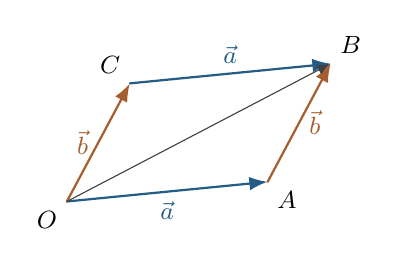
\begin{tikzpicture}[font=\small,>=Latex,line cap=round,line join=round]

\coordinate (O) at (0,0); \coordinate (A) at (2.55,.25);
\coordinate (C) at (.8,1.5); \coordinate (B) at (3.35,1.75);
\draw[->,curveblue,thick] (O)--node[below]{$\vec a$}(A);
\draw[->,curveblue,thick] (C)--node[above]{$\vec a$}(B);
\draw[->,accent,thick] (O)--node[left]{$\vec b$}(C);
\draw[->,accent,thick] (A)--node[right]{$\vec b$}(B);
\draw[->,black!75] (O)--(B);
\node[below left] at (O) {$O$};\node[below right] at (A) {$A$};
\node[above left] at (C) {$C$};\node[above right] at (B) {$B$};
\end{tikzpicture}
\end{document}
